Minha mãe era professora normalista e começou sua carreira como todas começavam na época, numa escola rural. 
Meu pai nunca aceitou que ela trabalhasse fora de casa, mas, com a ajuda de políticos, mamãe conseguiu que criassem para ela uma vaga na Fazenda Barrinha, que pertencia ao Tio Zé Amaral, marido da Tia Yolanda, irmã mais velha do papai. 
O plano era levar  meu irmão e eu junto com ela, pois o regulamento para ingresso na carreira exigia que ela estagiasse numa escola rural por pelo menos um ano até que fosse possível tentar uma transferência para a cidade. 
Papai permaneceria em casa e nos visitaria nos finais de semana. 
Tudo acertado, com a relutante concordância do marido, mamãe convocou a Vó Didi para providenciar nossos trajes de roça. 
As duas foram para a rua e pouco tempo depois voltaram sobraçando uma peça de brim azul-marinho. 
Rapidamente vovó desmanchou-a e tornou a dobrá-la em pregas largas sobre as quais recortou assim uma espécie de mamulengo com as nossas medidas, meia peça para cada um. 
Isso feito, sentou-se à máquina de costura e, em algumas horas, Reginaldo e eu envergávamos uma versão pioneira do macacão celebrizado, anos mais tarde, pela Revolução Cultural de Mao Tsé-Tung, na China. 
Para completar a elegância, ganhamos dois pares de Alpargatas Roda cada um, uma sapatilha de lona e corda usada pelos trabalhadores da lavoura naquele tempo. 
No dia seguinte, lá fomos nós de mala e cuia para a Barrinha.
                     
A escola era um comprido barracão de madeira apoiado sobre um baldrame de tijolos, para impedir a entrada de cobras. 
Tinha um odor peculiar de que me lembro até hoje, mistura de madeira seca com pó de giz, acrescido do cheiro de picumã que as crianças traziam na roupa por causa da fumaça dos fogões de lenha que as mal ventiladas casas da colônia não conseguiam dispersar. 
Do depósito de selas e tralhas contíguo à sala de aula, vinha se juntar o bodum de couro suado do lombo dos animais. 
Mas a escola, como tudo o que rodeava Tia Yolanda, era limpíssima, lavada e esfregada com soda. Na mesa, um vaso sobre a toalha bordada e engomada com esmero, aguardava o ramalhete improvisado colhido pelos alunos ao longo do caminho.  


\begin{figure}[H]
\centering
\includegraphics[width=0.4\linewidth]{5/mamãe+reginaldo.png}
\caption{Mamãe, Reginaldo e eu diante.}
\end{figure}

\begin{figure}[H]
\centering
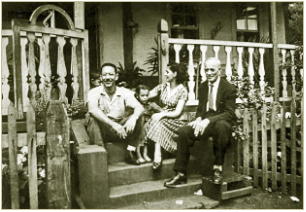
\includegraphics[width=0.6\linewidth]{5/papai+vô joão.png}
\caption{Papai e Vô João nos visitando na sede da fazenda.}
\end{figure}

O primeiro dia de aula numa escola rural tinha que ser invariavelmente dedicado a examinar as unhas, o cabelo e as mãos da criançada.
Piolho, unha suja, pescoço encardido, bicho de pé, nada escapava ao rigoroso escrutínio da brigada sanitária integrada pela minha mãe e pelo casal de tios. 
Na beira do poço, um a um, os alunos iam sendo examinados, lavados e escovados para aprender como deviam se apresentar diante da professora dali em diante. 
Era a primeira lição.

Olhando aqueles meninos atentos e obedientes à minha mãe, que chegavam alegres como uma revoada de andorinhas apesar da dura batalha de todos os dias para vencer os esses e erres, para imitar o talhe impecável da letra da professora, para desvendar os mistérios das divisões e multiplicações, é que eu comecei a achar que essa história de estudo devia ser muito importante mesmo. 
Mas, como esperar que mantivessem os cadernos limpos e organizados como minha mãe queria, se naquele lugar não havia como se livrar da terra nas mãos, nas roupas, na cara, em toda parte? 
Pois não é que eles acabavam conseguindo?  
O ano mal ia a meio e a maioria deles já tinha uma letra redonda e ligeiramente inclinada, como queria a professora, os cadernos encapados, com os parágrafos, margens e vinhetas apropriadamente distribuídos. 
Minha mãe era brava, mas vibrante, entusiasmada e gostava de cantar com eles. 
Também sabia fazer bonitos desenhos na lousa para ilustrar os temas das aulas. Talvez por isso, mais do que atenção, medo ou respeito, o que eu via na expressão daquelas crianças era gratidão, quase adoração.

\begin{figure}[H]
\centering
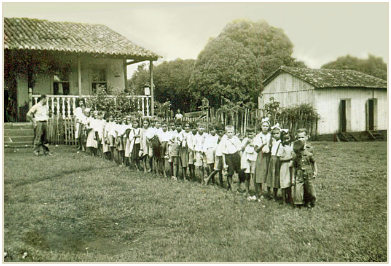
\includegraphics[width=0.6\linewidth]{5/escola.png}
\caption{Os alunos da Fazenda Barrinha, Reginaldo e eu à frente.}
\end{figure}

Foi naquela humilde escolinha rural da Fazenda Barrinha que, sem me dar conta, encantei-me pelo ofício de ensinar.  
E de aprender. 
Era fascinante observar como aquelas crianças, pouco mais que animaizinhos mudos e assustados no primeiro dia de aula, iam se afirmando na sua humanidade, à medida que progrediam nos estudos. 
Pareciam mais alegres, mais confiantes, como se as porteiras do mundo fossem se abrindo diante deles e aquele ingênuo desenho da estrada florida e ensolarada que estampava as capas dos cadernos baratos que o governo lhes fornecia, fosse se materializando diante dos seus olhos.  
Por causa disso, quando eu própria cheguei à idade de frequentar a escola, tinha desse universo a melhor das impressões.
    
A hoje pejorativamente chamada escola reprodutivista, de inspiração cartesiana, tinha o efeito de tornar o mundo muito simples e seguro para as crianças daquele tempo. 
Quem duvidaria que o Brasil fora descoberto por culpa das calmarias na costa africana, se quem o afirmava era Dona Anahyde, minha professora de 4ª série, corpulenta senhora de cabelos vermelhos colados à testa em caprichadas ondinhas e expressão feroz de um guarda penitenciário? 
Aliás, como mamãe proclamava orgulhosamente, fiz meu primário com as melhores professoras do Grupo Escolar, a começar por ela própria, o que significava, principalmente, ter experimentado as mais rígidas disciplinadoras da casa. 
Tenho certeza de que ao cabo da minha vida, a última coisa a se apagar na memória serão os nomes das cidades percorridas pela Estrada de Ferro Central do Brasil, decorados no dia em que Tia Odete, que se gabava de ouvir um alfinete cair na sua silente classe de 3º ano, manteve-me em pé diante do mapa da dita ferrovia durante a tarde toda, porque olhei para trás durante suas explicações, ao ter o cabelo puxado por meu irmão. 
O mundo se dividia, claramente, entre o certo e o errado, o bem e o mal, sem atenuantes, sem nuances, sem relativismos, sem dúvidas. 
Havia uma resposta correta para tudo e a resposta era aquela da professora. 
E os pais estavam de pleno acordo quanto a isso. 
Portanto, podíamos brincar despreocupados no recreio. A vida era previsível e se alguém tivesse cabeça boa para decorar e obedecer a regras e instruções, não havia o que temer. 

Um dia, já Coordenadora Pedagógica de um colégio jesuíta no Piauí, desci aos porões do centenário prédio atrás de livros antigos de aritmética. 
Remexendo as estantes empoeiradas do arquivo, encontrei, caído por detrás delas, um grande caderno de gravuras que o Ministério da Educação distribuía, até meados do século XX, por todas as salas de aula do país e que eu vi, pela primeira vez, na escola da Barrinha.  
Era o material de apoio utilizado nas aulas de redação, numa prática anunciada como “composição à vista de uma gravura” e que podia ser, alternadamente, uma descrição ou uma narração. 
Consistia numa sucessão de estampas ingênuas, exibindo crianças e animaizinhos felizes em campos floridos, árvores frondosas, casinhas aninhadas entre montanhas, nuvens brancas e gorduchas por sobre as quais brilhavam invariavelmente os raios amarelos do sol. 
Judiciosamente, a professora dava o começo, escrito em letras caprichadas na lousa: “Era uma linda manhã de primavera\dots”. 
As reticências eram a deixa para que nós, os alunos, fôssemos em frente. 
Maravilhada, corri para exibir o achado à minha colega de Coordenação, Jovina, que tinha mais ou menos a minha idade e, portanto, devia ter cursado o primário na mesma época.  
Paulista eu, piauiense ela, descobrimos, às gargalhadas, que a distância de alguns milhares de quilômetros não impedira a inacreditável coincidência de adjetivos, advérbios e frases feitas inspiradas pelas tais gravuras e que, usados em profusão, garantiram para ambas a aprovação com louvor naquela matéria. Assim que passou o surto de hilaridade, minha colega comentou: 

{\small\itshape``-- Hoje a gente ri, mas me diga, aqui na escola, quando é preciso redigir um discurso, um ofício, um requerimento ou até uma simples comunicação, é atrás de nós duas que eles vêm, é, ou não é?''}